\documentclass{article}

% NeurIPS 2026 Evaluations & Datasets track, anonymous submission.
\usepackage[eandd]{neurips_2026}

\usepackage[utf8]{inputenc}
\usepackage[T1]{fontenc}
\usepackage[hypertexnames=false]{hyperref}
\usepackage{url}
\usepackage{booktabs}
\usepackage{amsmath}
\usepackage{amsfonts}
\usepackage{amssymb}
\usepackage{graphicx}
\usepackage{float}
\usepackage{microtype}
\usepackage{xcolor}
\usepackage{enumitem}
\usepackage{multirow}
\usepackage{array}
\hypersetup{hidelinks}
\raggedbottom

\title{PhysEval: Quantitative Physical Evaluation for Text-to-Video World Generation}

\author{Anonymous Authors}

\newcommand{\bench}{PhysEval}
\newcommand{\todo}[1]{\textcolor{red}{[TODO: #1]}}
\newcommand{\relerr}{\operatorname{RelErr}}
\newcommand{\score}{\operatorname{Score}}
\newcommand{\eps}{\varepsilon}
\newcommand{\cmark}{\checkmark}
\newcommand{\figtodo}[2]{%
\begin{figure}[H]
\centering
\fbox{\begin{minipage}{0.92\linewidth}
\vspace{0.75em}
\textbf{Figure placeholder.} #2
\vspace{0.75em}
\end{minipage}}
\caption{#1}
\end{figure}}

\begin{document}

\maketitle

\begin{abstract}
Text-to-video (T2V) generation has advanced rapidly, yet evaluating whether generated motion obeys specified physical quantities remains challenging.
Most existing benchmarks emphasize perceptual quality, text-video alignment, or qualitative physical plausibility, leaving it unclear whether a visually plausible video can support a numerical physical measurement.
To this end, we present \bench{}, a benchmark dataset and automatic evaluation protocol for quantitative physical evaluation of T2V world generation.
\bench{} pairs each prompt with auditable metadata, including the target value, unit, evaluator type, expected object count, calibration setting, and known physical parameters.
It covers ten physical metrics across kinematics, gravity, material and interaction parameters, and conservation laws.
For each generated video, the evaluation pipeline performs object tracking, trajectory extraction, mask-reliability estimation, task-specific inverse physical measurement, and effective-video scoring.
Together, tracking validity, physics validity, and mask reliability identify which generated videos are effective under the benchmark protocol and determine an adjusted score for evaluating physical accuracy.
This design evaluates physical correctness on measurable generations while still exposing why other samples cannot be used as valid physical evidence.
\end{abstract}

\section{Introduction}

Recent T2V systems have improved rapidly in visual fidelity, prompt following, and short-term temporal coherence.
However, a visually convincing video can still violate simple physical relationships.
A falling object may accelerate at the wrong rate, a sliding object may decelerate in a way that implies the wrong friction coefficient, a collision may lose or create momentum, or a spring-mass system may oscillate with an incorrect period.
For applications that use generated videos as scientific illustrations, simulation surrogates, robotics data, or educational material, this distinction matters: the video should not only look plausible, but should also support a physical measurement.

Most existing video-generation evaluations emphasize perceptual quality, text-video alignment, commonsense plausibility, or human preference.
Physics-aware benchmarks move closer to the needs of world simulation, but they often evaluate whether a physical phenomenon occurs rather than whether a generated trajectory matches a numerical target.
This leaves a gap between \emph{physical commonsense evaluation} and \emph{quantitative physical evaluation}.
The former asks whether the video looks physically reasonable; the latter asks whether a measurable physical quantity is correct.
\bench{} targets this second setting.

The key idea of \bench{} is to make each prompt auditable through a structured benchmark specification.
The prompt is used for generation, but evaluation is controlled by structured fields containing the metric, target value, unit, expected number of objects, calibration information, and known physical constants.
This design makes the benchmark less dependent on subjective judgments and more robust to ambiguous language.
The same generated video can be inspected through its trajectory, mask stability, object count, evaluator status, target value, measured value, and final score.

\begin{figure}[H]
\centering
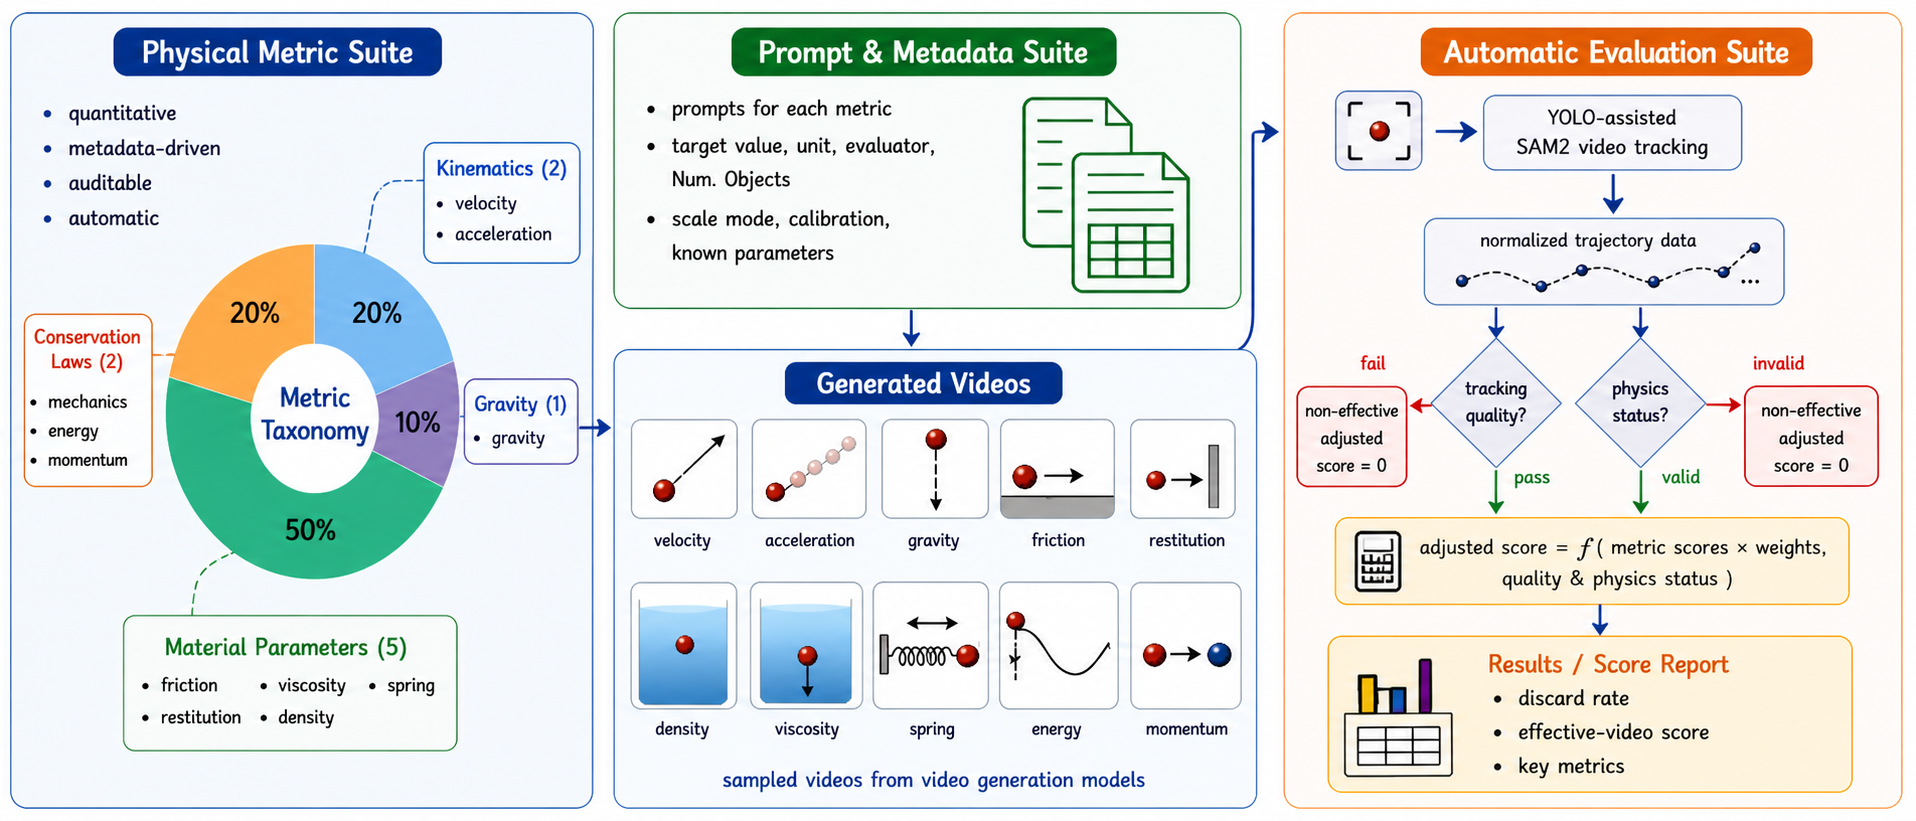
\includegraphics[width=\linewidth]{figures/fig1_benchmark_overview.png}
\caption{Overview of \bench{}. \bench{} organizes quantitative physical evaluation into a physical metric suite, a prompt and metadata suite, and an automatic evaluation suite. Each metric is paired with prompts and auditable metadata, generated videos are sampled from T2V models, and YOLO-assisted SAM2 tracking with task-specific physics evaluators produces discard diagnostics and effective-video scores for measuring physical accuracy.}
\label{fig:benchmark-overview}
\end{figure}

Our main quantitative analysis uses effective-video scoring.
The effective-video score measures physical accuracy on videos that are measurable under the protocol, and therefore directly answers whether a model's measurable motions match the requested physical values.
Discard rate is reported alongside this score to indicate how often a model fails to produce measurable samples.
This separation prevents static or untrackable videos from being ignored, while keeping the main ranking focused on physical accuracy among measurable generations.

Our contributions are:
\begin{itemize}[leftmargin=1.3em]
    \item We introduce \bench, a benchmark for quantitative physical evaluation of T2V generation.
    \item We define a structured benchmark specification that links prompts to target physical values, evaluator types, calibration, expected object counts, and known parameters.
    \item We implement a batch evaluation pipeline that combines object initialization, mask tracking, trajectory extraction, tracking-quality checks, mask-quality scoring, and task-specific physical estimators.
    \item We propose an effective-video-centered scoring protocol that separates physical accuracy, estimation validity, tracking quality, mask reliability, and discard diagnostics.
    \item We provide diagnostic signals for discard analysis and reliability analysis, including invalid physical fits, wrong object counts, nearly static motion, and mask-instability scores.
\end{itemize}

\section{Related Work}

\subsection{General and Compositional Video Evaluation}

Video-generation benchmarks first focused on broad quality and alignment signals.
VBench decomposes video generation quality into hierarchical perceptual and semantic dimensions, including subject consistency, motion smoothness, temporal flickering, aesthetic quality, and text-video consistency~\citep{huang2023vbench}.
T2V-CompBench studies compositional text-to-video generation with MLLM-based, detection-based, and tracking-based metrics for attribute binding, spatial relationships, motion binding, action binding, object interactions, and numeracy~\citep{sun2025t2vcompbench}.
These benchmarks are useful for evaluating whether a video is coherent and follows a prompt, but their metrics do not measure whether a generated motion corresponds to a specified physical value.

\subsection{Physical Commonsense Benchmarks}

Physics-aware benchmarks move closer to world simulation by asking whether generated videos obey intuitive physical commonsense.
VideoPhy curates real-world physical activity prompts and evaluates both semantic adherence and physical plausibility~\citep{bansal2024videophy}.
PhyGenBench organizes prompts around physical laws across mechanics, optics, thermal processes, and material properties, and evaluates generated videos with a hierarchical VLM/LLM-based framework~\citep{meng2024phygenbench}.
These works expose failures that ordinary visual-quality metrics miss, but their evaluation target is usually qualitative or categorical: whether the expected physical phenomenon appears plausible, rather than whether a trajectory implies a requested numerical quantity.

\subsection{Quantitative and World-Model Physics Benchmarks}

Recent benchmarks introduce more explicit physical diagnostics, especially in image- or video-conditioned world-model settings.
Morpheus evaluates video generative models using real physical experiments and physics-informed scores based on conservation invariants and equation fitting~\citep{zhang2025morpheus}.
However, this style of evaluation depends on physical experiment data and per-sample physical setup information, so it is not a pure text-to-video benchmark.
WorldBench emphasizes concept-specific evaluation and includes physical-parameter diagnostics for quantities such as gravity, friction, and viscosity~\citep{upadhyay2026worldbench}.
4DWorldBench further broadens evaluation to multimodal 3D/4D world generation, combining perceptual quality, condition alignment, physical realism, and 4D consistency~\citep{lu2025fourDworldbench}.
\bench{} is complementary to these efforts: it targets T2V outputs directly, uses prompts with explicit numerical physical targets, and automatically estimates those targets from generated videos through object tracking and task-specific inverse physics.

\begin{table}[H]
\centering
\scriptsize
\setlength{\tabcolsep}{2pt}
\caption{Comparison with representative benchmarks. ``Auto.'' means that the benchmark can score generated videos without per-video human labels or manual physical annotations at evaluation time.}
\label{tab:benchmark-comparison}
\begin{tabular}{@{}>{\raggedright\arraybackslash}p{0.22\linewidth}>{\centering\arraybackslash}p{0.17\linewidth}>{\centering\arraybackslash}p{0.16\linewidth}>{\centering\arraybackslash}p{0.18\linewidth}>{\centering\arraybackslash}p{0.13\linewidth}>{\centering\arraybackslash}p{0.08\linewidth}@{}}
\toprule
Benchmark & Primary setting & Physical focus & Quant. physical measurement & Auto. & T2V \\
\midrule
VBench~\citep{huang2023vbench} & Text-to-video & partial & -- & \cmark{} & \cmark{} \\
T2V-CompBench~\citep{sun2025t2vcompbench} & Text-to-video & partial & -- & \cmark{} & \cmark{} \\
VideoPhy~\citep{bansal2024videophy} & Text-to-video & commonsense & -- & partial & \cmark{} \\
PhyGenBench~\citep{meng2024phygenbench} & Text-to-video & commonsense & -- & \cmark{} & \cmark{} \\
Morpheus~\citep{zhang2025morpheus} & conditioned video generation & physical invariants & \cmark{} & partial & -- \\
WorldBench~\citep{upadhyay2026worldbench} & constrained video prediction & physical parameters & partial & \cmark{} & -- \\
\bench{} & Text-to-video & physical quantities & \cmark{} & \cmark{} & \cmark{} \\
\bottomrule
\end{tabular}
\end{table}

\section{Benchmark Datasets}

\bench{} is organized around a simple principle: every video should be tied to a physical quantity that can be measured from tracked motion.
Inspired by physics-aware benchmark construction that isolates clear phenomena and physical laws~\citep{meng2024phygenbench}, our dataset avoids prompts that require multiple unrelated physical effects to be judged at once.
Instead, each instance has one primary evaluator and one target value.
This makes the output of the benchmark interpretable: the evaluator either measures the specified quantity, marks the video as weakly valid, or reports why the measurement failed.

\subsection{Physical Task Taxonomy}

The current benchmark covers kinematics, physical-constant estimation, material-parameter estimation, and conservation-style tasks.
Kinematics includes velocity and acceleration.
Gravity is treated as a separate physical constant because the evaluator estimates a scene-level acceleration due to gravity rather than a generic object acceleration.
Material and interaction parameters include friction coefficient, restitution coefficient, density, fluid viscosity, and spring constant.
Conservation tasks include mechanical energy conservation and one-dimensional momentum conservation.
These categories were chosen because they can be estimated from short monocular videos under controlled assumptions, while still requiring nontrivial object motion and temporal consistency.
The resulting measurements rely on idealized physical models; the dataset specification below states the main planar-motion constraint, and Appendix~\ref{app:idealizations} lists the modeling assumptions used by the inverse calculations.

\begin{table}[H]
\centering
\scriptsize
\setlength{\tabcolsep}{2pt}
\caption{Task taxonomy. The final paper should replace counts with the final benchmark statistics.}
\label{tab:task-taxonomy}
\begin{tabular}{@{}>{\raggedright\arraybackslash}p{0.18\linewidth}>{\raggedright\arraybackslash}p{0.23\linewidth}>{\centering\arraybackslash}p{0.12\linewidth}>{\raggedright\arraybackslash}p{0.38\linewidth}@{}}
\toprule
Category & Metric & Expected objects & Measured quantity \\
\midrule
Kinematics & Velocity & 1 & Linear slope \\
Kinematics & Acceleration & 1 & Quadratic coefficient \\
Physical constants & Gravity & 1 & Free-fall acceleration \\
Material & Friction coefficient & 1 & Deceleration ratio \\
Material & Restitution coefficient & 1 & Speed ratio \\
Material & Density & 1 & Early acceleration \\
Material & Fluid viscosity & 1 & Terminal velocity \\
Material & Spring constant & 1 & Oscillation period \\
Conservation & Mechanical energy conservation & 1 & Energy ratio \\
Conservation & Momentum conservation 1D & 2 & Momentum error \\
\bottomrule
\end{tabular}
\end{table}

\subsection{Dataset Specification}

Each benchmark instance specifies the prompt identifier, natural-language prompt, metric name, target value, target unit, evaluator name, expected object count, calibration mode, frame-rate assumption, and optional known parameters such as gravity, mass, object radius, fluid density, or scale.
This specification follows the task taxonomy in Table~\ref{tab:task-taxonomy}, while Figure~\ref{fig:prompt-construction} illustrates how category information is converted into prompts and evaluation metadata.
The expected object count is important because many physical tasks are only meaningful if the generated video contains the correct number of trackable objects.
For example, a two-object momentum task cannot be measured if the tracker finds only one persistent object; a one-object acceleration task should not accidentally track a second distractor as part of the target.

Because the current evaluators estimate physical quantities from 2D image trajectories and benchmark-provided scale information, each prompt is written under a fixed-camera, approximately planar-motion assumption.
In practice, this means that the prompt should ask for a stable camera and object motion in a plane approximately parallel to the image plane.
Generated videos may still violate this instruction through depth drift, apparent scale change, or unstable masks.
For this reason, \bench{} uses a mask-derived reliability term, denoted by $Q_{\mathrm{mask}}$ in the scoring equations, as a soft proxy for whether the 2D measurement is trustworthy.
Appendix~\ref{app:mask-quality} gives the detailed definition and thresholds, while Appendix~\ref{app:idealizations} states the physical modeling assumptions used by the inverse calculations.

\begin{figure}[H]
\centering
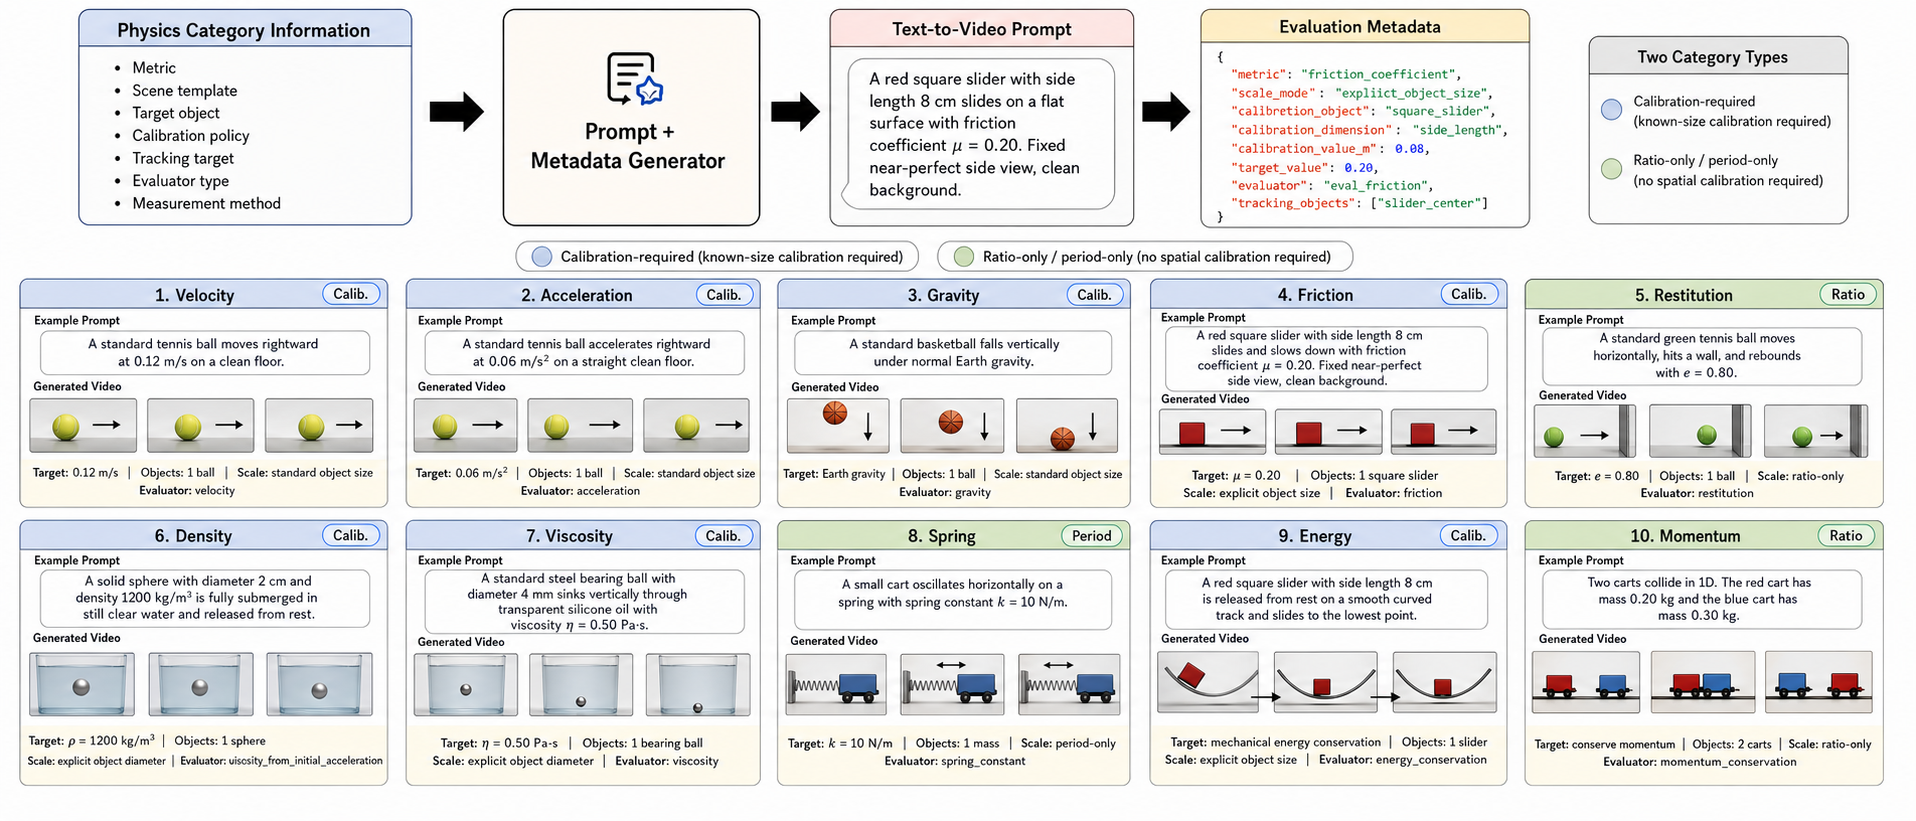
\includegraphics[width=\linewidth]{figures/fig2_prompt_construction.png}
\caption{Prompt construction process and examples across physical categories. \todo{Temporary figure; redraw or polish before final submission.}}
\label{fig:prompt-construction}
\end{figure}

For each generated video, the pipeline produces a compact evaluation record containing the benchmark specification, physical evaluator output, tracking-quality status, mask-quality diagnostics, target value, measured value, relative error, and reason tokens.
This compact record is intentional: one video should be explainable through its measured trajectory, diagnostic plots when needed, and a small set of interpretable status fields.
The same organization also makes model-level scoring simple, since per-video records can be aggregated into model-level and metric-level summaries.

\section{Evaluation}

The effective set is defined by two hard validity conditions: tracking quality and physics-estimation validity.
A video is effective only when the tracker returns the expected measurable motion and the task-specific evaluator returns \texttt{valid} or \texttt{weak\_valid}.
The implementation may check tracking first to avoid unnecessary downstream computation on untrackable videos, but conceptually these are parallel requirements for measurability.
For diagnostic analysis, we therefore report videos that fail only tracking, fail only physics estimation, or fail both.
Only after both gates are satisfied does the scorer compute the mask-quality multiplier, relative error, physical-accuracy score, and adjusted final score.
This design keeps tracking failures, physical-fitting failures, and mask reliability as distinct factors.

\subsection{Ordered Validity Gates}

Tracking quality is one of the two hard gates for effective videos.
The tracker is checked for expected object count, valid-frame coverage, and meaningful motion.
If the number of persistent objects differs from the expected count in the benchmark specification, the video receives \texttt{object\_count\_mismatch}.
If the primary object moves less than the configured number of object diameters, it receives \texttt{no\_meaningful\_motion}.
By default, tracking failures make the video ineffective and assign an adjusted score of zero:
\begin{equation}
    M_{\mathrm{track}} =
    \begin{cases}
    1, & \text{tracking passes},\\
    0, & \text{tracking fails under the hard-gate policy}.
    \end{cases}
\end{equation}
This prevents a nearly static video, a missing object, or a wrong-object track from being treated as a physical sample.

The physics-validity gate is the other hard gate for effective videos.
Each evaluator returns one of four statuses.
\texttt{valid} means the measurement is available and passes evaluator-specific checks.
\texttt{weak\_valid} means a measurement exists but some fit, event, or monotonicity condition is weak.
\texttt{invalid} and \texttt{failed} mean the measurement should not be used.
The current score uses multipliers:
\begin{equation}
    M_{\mathrm{valid}} =
    \begin{cases}
    1.0, & \texttt{valid},\\
    0.75, & \texttt{weak\_valid},\\
    0, & \texttt{invalid} \text{ or } \texttt{failed},
    \end{cases}
\end{equation}

Mask quality is computed only after a video satisfies both tracking quality and physics validity.
It is a continuous reliability score in $[0,1]$ derived from mask-area variation, bounding-box variation, area jumps, trend strength, translation-aligned IoU, centroid-step size, and middle-window coverage.
The default protocol uses mask quality as a soft reliability multiplier rather than a hard exclusion criterion:
\begin{equation}
    M_{\mathrm{measure}} = M_{\mathrm{track}} \cdot Q_{\mathrm{mask}}.
\end{equation}
Tracking quality and physics validity jointly decide whether a video is measurable, while mask instability expresses how reliable the measurement is.
Severe mask failures can drive the adjusted score close to zero, but they do not reduce the effective-video count unless the user explicitly chooses a stricter policy.

\subsection{Scoring Formula}

For a target value $y$ and measured value $\hat{y}$, we compute
\begin{equation}
    \relerr = \frac{|\hat{y}-y|}{\max(|y|,\eps)}.
\end{equation}
The base score is an exponentially decaying function of relative error:
\begin{equation}
    S_{\mathrm{phys}} = 100 \exp(-\relerr / \tau_k),
\end{equation}
where $\tau_k$ is a metric-specific tolerance.
Larger $\tau_k$ values make the score more forgiving.
The default tolerances are intentionally moderate because generated videos often contain small scale, timing, and tracking noise; the exact values must be reported with the results.

\begin{table}[H]
\centering
\scriptsize
\caption{Default tolerance values used in the scoring protocol. These values can be reported as global settings or specified separately for each metric.}
\label{tab:tau}
\begin{tabular}{lc@{\hspace{1.5em}}lc}
\toprule
Metric & $\tau_k$ & Metric & $\tau_k$ \\
\midrule
Velocity & 0.30 & Acceleration & 0.35 \\
Gravity & 0.30 & Friction coefficient & 0.35 \\
Restitution coefficient & 0.30 & Density & 0.35 \\
Fluid viscosity & 0.40 & Spring constant & 0.35 \\
Mechanical energy conservation & 0.35 & Momentum conservation 1D & 0.35 \\
\bottomrule
\end{tabular}
\end{table}

The adjusted per-video score is
\begin{equation}
    S_{\mathrm{video}} =
    S_{\mathrm{phys}} \cdot M_{\mathrm{valid}} \cdot M_{\mathrm{measure}}.
\end{equation}
A video is included in the effective set if and only if it satisfies both hard gates: (1) tracking passes under the selected tracking policy; and (2) the evaluator status is \texttt{valid} or \texttt{weak\_valid}.
Only after these two gates pass does the scorer require a computable numerical physical score.
The effective-video score is the mean adjusted score over this effective set and is the primary score used for physical-accuracy analysis.
The discard rate is
\begin{equation}
    R_{\mathrm{discard}} = 1 - \frac{N_{\mathrm{effective}}}{N_{\mathrm{total}}}.
\end{equation}
For diagnostic reporting, we distinguish videos that fail tracking only, fail physics validity only, or fail both gates.

\section{Experiments}

\subsection{Experiment Setup}

Following the reporting style of recent T2V physics benchmarks, we describe the generation setup in prose rather than using a placeholder setup table.
All evaluated systems use the same benchmark specification, prompt text, video naming convention, tracking configuration, physical evaluators, and scoring policy.
For each model, we generate videos for the full prompt set and evaluate them with the same ordered protocol.
The pipeline first produces per-video evaluation records and then aggregates them into model-level and metric-level summaries.

The final version will state the evaluated model names and versions, generation dates, resolution, duration, frame rate, sampling settings, number of generations per prompt, retry policy, and whether any failed generations are counted as zero.
Generated videos are not manually filtered before scoring.
\todo{Fill in final evaluated model list and generation settings in prose.}

\subsection{Discard Rate}

Discard analysis is essential context for interpreting effective-video scores.
A high effective-video score with a high discard rate means that the model can be physically accurate when it generates measurable videos, but often fails to produce samples that the protocol can evaluate.
A lower effective-video score with a low discard rate may indicate a model that reliably generates measurable motion but does not match the target physical values.
Therefore, our main analysis reports effective-video scores together with discard rates, so physical accuracy and measurability remain distinguishable.

Because tracking quality and physics validity are parallel requirements for effective videos, the discard-rate analysis separates discarded videos into three diagnostic cases:
\begin{itemize}[leftmargin=1.3em]
    \item \textbf{tracking only}: tracking fails, while the physics evaluator status is \texttt{valid} or \texttt{weak\_valid};
    \item \textbf{physics only}: tracking passes, while the physics evaluator status is \texttt{invalid} or \texttt{failed};
    \item \textbf{both}: tracking fails and the physics evaluator status is also \texttt{invalid} or \texttt{failed}.
\end{itemize}

\figtodo{Average discard rates across physical experiments.}
{Insert a stacked bar chart at this position, following the style of the provided reference image. The x-axis should list models; the y-axis should be discard rate. Stack the bars by diagnostic source: tracking only, physics only, and both tracking and physics. Mask quality should not appear as a discard type under the default policy because it is a soft multiplier. Grouping by task family or frame setting can be added only if the final experiment design requires it. The caption should emphasize that discard rate is contextual information for interpreting effective-video scores.}

Figure 3 should be read as a measurability analysis rather than a physical-accuracy ranking.
A model with a high discard rate may still achieve strong effective-video scores on the subset that remains, but it produces valid measurable videos only with limited probability.
This distinction is important for text-to-video evaluation: a model may occasionally generate trajectories that match the requested physical quantity, while still frequently producing static clips, ambiguous object appearances, unstable tracking targets, or motions that are not suitable for numerical fitting.
The stacked decomposition further indicates where failures arise.
A tracking-only dominated bar points to visual or temporal issues that prevent reliable object localization.
A physics-only dominated bar means that the object can be tracked, but the measured trajectory is inconsistent with the target physical value or lacks enough usable dynamic signal for fitting.
A large overlap indicates the strongest failure mode, where the video is both difficult to track and physically invalid under the evaluator.
We therefore use discard rate to qualify effective-video scores: effective-video scores measure accuracy conditional on measurability, while discard rates show how often each model reaches that measurable regime.

\subsection{Quantitative Evaluation}

The quantitative evaluation is centered on effective-video scoring.
This score measures physical accuracy only on videos that pass the tracking and physics-validity gates.

\begin{table}[H]
\centering
\scriptsize
\setlength{\tabcolsep}{3pt}
\caption{Effective-video scores by physical metric, normalized to $[0,1]$ for display. Scores are computed only over videos that satisfy both hard gates: tracking quality and \texttt{valid} or \texttt{weak\_valid} physics status. Values below 0.5 are shown as $<0.5$, and the best model for each metric is bolded. \todo{Replace placeholder values with final results.}}
\label{tab:effective-metric-scores}
\begin{tabular}{lcccccccccc}
\toprule
Model & Vel. & Acc. & Grav. & Fric. & Rest. & Dens. & Visc. & Spring & Energy & Mom. \\
\midrule
Wan2.2 & \textbf{0.74} & \textbf{0.68} & \textbf{0.71} & $<0.5$ & \textbf{0.63} & \textbf{0.52} & $<0.5$ & \textbf{0.58} & \textbf{0.61} & $<0.5$ \\
Jimeng & 0.69 & $<0.5$ & 0.65 & \textbf{0.57} & $<0.5$ & $<0.5$ & \textbf{0.54} & $<0.5$ & 0.56 & \textbf{0.52} \\
\bottomrule
\end{tabular}
\end{table}

\subsection{Metric and Model Analysis}

The effective-video scores in Table~\ref{tab:effective-metric-scores} should first be read across metrics.
Across models, kinematic quantities and simple gravitational motion are expected to be relatively stronger because they involve a single visible object, a clear motion direction, and comparatively direct trajectory fitting.
Interaction and material parameters are more demanding.
Friction, restitution, density, viscosity, and spring constant require the video to preserve a specific event structure, object scale, timing, and monotonic or periodic motion over enough frames for fitting.
Conservation metrics are often harder still, because they depend on multi-object consistency or energy-state consistency rather than a single object's smooth trajectory.
When several models score poorly on the same physical quantity, the result suggests a benchmark-wide difficulty rather than a model-specific weakness: the current T2V systems may generate visually plausible motion while missing the quantitative cues needed for that physical law or parameter.
\todo{Replace this trend discussion with the final empirical ranking once all results are available.}

\figtodo{Effective-video radar comparison across models.}
{Insert a radar chart using only effective-video scores. Each axis should correspond to one physical metric, and each model should be drawn as a separate colored polygon. Use the same normalized $[0,1]$ scale as Table~\ref{tab:effective-metric-scores}. The figure should make it easy to compare model profiles: broad polygons indicate balanced physical accuracy on measurable videos, while narrow or uneven polygons indicate metric-specific strengths and weaknesses.}

Figure 4 complements the table by showing the shape of each model's effective-video performance profile.
A model with a broad and balanced radar area is not merely strong on one isolated task; it is more consistently accurate across different physical quantities after invalid videos are removed.
A model with sharp peaks may handle a subset of phenomena, such as simple kinematics or one material parameter, while still failing on tasks that require event timing, object interaction, or reliable scale interpretation.
Model differences should therefore be interpreted both by average score and by profile shape.
For example, one model may lead on velocity, acceleration, and gravity because it produces smoother single-object trajectories, while another may be more competitive on friction or viscosity if it better expresses gradual slowing or fluid resistance.
The final analysis will replace these examples with measured model-specific differences.

End-to-end scores are kept out of the main comparison because they combine two effects: whether a video is measurable and whether the measured physical value is accurate.
For completeness, we report them separately in \hyperref[app:end-to-end-scores]{Appendix~\ref{app:end-to-end-scores}}.

\section{Discussion}

\bench{} focuses on short monocular videos under controlled benchmark conditions.
This scope makes quantitative physical evaluation feasible, but it does not cover all forms of physical realism.
Important extensions include deformable bodies, complex fluids, camera motion, occlusion-heavy scenes, multi-view consistency, and long-horizon interactions.
Expanding the benchmark in these directions would require richer scene specifications and evaluators that can reason beyond simple image-plane trajectories.

The benchmark depends on automatic tracking and segmentation.
Although tracking-quality gates and mask-quality scores expose many failures, a small number of videos may still be mismeasured.
Mask quality is also only an indirect indicator of the planar-motion assumption; true 3D reconstruction would be needed to fully verify depth motion.
Future versions could incorporate stronger trackers, explicit uncertainty estimates, multi-view reconstruction, or human-audited subsets to better quantify measurement error.

The physical evaluators rely on simplified models.
For example, friction assumes interpretable sliding deceleration, fluid viscosity uses a terminal-velocity approximation, and conservation tasks assume a detectable event window.
These simplifications are deliberate because they make T2V outputs measurable, but they limit the types of prompts that can be scored reliably.
Future work can add evaluators for richer dynamics while preserving the benchmark's central requirement: every reported score should correspond to an auditable physical quantity.

\section{Conclusion}

We introduced \bench, a benchmark for quantitative physical evaluation of T2V generation.
Unlike broad perceptual benchmarks or physical commonsense benchmarks, \bench{} asks whether generated videos match specified physical values.
The pipeline produces auditable per-video evaluation records containing target values, measured values, physical statuses, tracking diagnostics, mask scores, and exclusion reasons.
The scoring protocol centers on effective-video scores and uses discard diagnostics to separate physical accuracy from the ability to generate measurable videos.
\todo{Replace with final empirical conclusion after all model scores are available.}

{\small
\bibliographystyle{plainnat}
\bibliography{references}
}

\appendix

\section{Physical Modeling Assumptions}
\label{app:idealizations}

The inverse physical estimates in \bench{} are intentionally based on simple, auditable models.
This makes the benchmark interpretable, but it also means that each evaluator is valid only under a small set of idealized conditions.
The benchmark prompts are written to encourage these conditions, and the tracking and physics-validity gates reject videos that visibly violate them.

\paragraph{Shared assumptions.}
All evaluators assume a fixed camera, approximately planar motion, a known or inferable time base, and a stable 2D object track.
When metric units are reported, the evaluator also assumes that the benchmark-provided scale is appropriate for the visible plane of motion.
The object is treated as a rigid body unless the task explicitly concerns material or fluid behavior.

\paragraph{Kinematics and gravity.}
Velocity and acceleration estimates assume that the tracked center is a reasonable proxy for the object's physical position.
The gravity evaluator assumes free-fall-like motion in the visible vertical direction, negligible air resistance over the short observed interval, and no hidden support force after release.
Videos with strong perspective drift, depth motion, or non-free-fall events are therefore not appropriate samples for this evaluator.

\paragraph{Friction and restitution.}
The friction evaluator assumes sliding along an approximately one-dimensional surface with a roughly constant kinetic friction coefficient.
It does not model rolling resistance, deformation, changing contact geometry, or active propulsion.
The restitution evaluator assumes an identifiable impact event against a fixed surface and estimates the coefficient from local pre- and post-impact speeds; it does not model spin, tangential friction, or multiple simultaneous contacts.

\paragraph{Density and viscosity.}
Density is estimated using an early falling interval in a fluid and assumes that the fluid is low-viscosity enough for drag to be negligible in the chosen early window.
This is why the benchmark should use liquids with relatively small viscosity for density prompts and avoid cases where terminal velocity is reached immediately.
The viscosity evaluator, in contrast, assumes a late terminal-velocity-like regime and applies a Stokes-style relation; this is most appropriate for small spherical objects, laminar flow, known radius, known densities, and low Reynolds number.

\paragraph{Spring, energy, and momentum.}
The spring evaluator assumes approximately harmonic motion with a stable period and known mass.
The mechanical-energy evaluator assumes that gravitational potential energy and translational kinetic energy dominate, so losses due to drag, rotation, deformation, and sound are ignored.
The momentum evaluator assumes a one-dimensional collision with known masses and a detectable pre/post-event window; it does not attempt to model hidden out-of-plane momentum or rotational transfer.

\section{Evaluator Details}

This appendix lists the formulas used by the current evaluators where the computation can be written compactly.
Let a tracked object have image centers $(x_i,y_i)$ at times $t_i$.
When a metric scale is available, let $\alpha$ denote meters per pixel.
For a chosen axis, the trajectory is projected to a one-dimensional coordinate $s_i$.
For a fixed axis, $s_i=\alpha x_i$ or $s_i=\alpha y_i$.
For automatic axis selection, the implementation uses the first principal component of the centered trajectory.
Linear and quadratic fits are least-squares fits:
\begin{align}
    (\hat{v},\hat{c}) &= \arg\min_{v,c}\sum_i (s_i-vt_i-c)^2,\\
    (\hat{a}_2,\hat{b},\hat{c}) &= \arg\min_{a_2,b,c}\sum_i (s_i-a_2t_i^2-bt_i-c)^2.
\end{align}
The fit quality reported by the evaluator is
\begin{equation}
    R^2 = 1 - \frac{\sum_i(s_i-\hat{s}_i)^2}{\sum_i(s_i-\bar{s})^2}.
\end{equation}

\paragraph{Velocity.}
The velocity evaluator fits $s_i\approx vt_i+c$ and reports
\begin{equation}
    \hat{y}_{\mathrm{vel}} = |\hat{v}|.
\end{equation}

\paragraph{Acceleration.}
The acceleration evaluator fits $s_i\approx a_2t_i^2+bt_i+c$ and reports
\begin{equation}
    \hat{y}_{\mathrm{acc}} = 2\hat{a}_2,
\end{equation}
or $|2\hat{a}_2|$ when the target acceleration is nonnegative.

\paragraph{Gravity.}
Gravity uses the vertical image coordinate with downward direction positive.
With $s_i=\alpha y_i$, the same quadratic fit gives
\begin{equation}
    \hat{g} = |2\hat{a}_2|.
\end{equation}
For ratio-only settings without metric scale, the same expression is reported in pixel units.

\paragraph{Friction coefficient.}
The friction evaluator first checks that the motion is approximately one-dimensional.
It then estimates sliding acceleration from the quadratic fit and computes
\begin{equation}
    \hat{\mu} = \frac{|2\hat{a}_2|}{\max(|g|,\eps)}.
\end{equation}
If the fitted trajectory does not show a decreasing speed trend, the result is marked \texttt{weak\_valid}.

\paragraph{Restitution coefficient.}
The restitution evaluator detects a velocity sign change as the collision event.
It fits local slopes before and after the event:
\begin{align}
    \hat{v}_{\mathrm{before}} &= \operatorname{slope}(s_{i-w:i-1}),\\
    \hat{v}_{\mathrm{after}} &= \operatorname{slope}(s_{i+1:i+w}).
\end{align}
The measured coefficient is
\begin{equation}
    \hat{e} = \frac{|\hat{v}_{\mathrm{after}}|}{\max(|\hat{v}_{\mathrm{before}}|,\eps)}.
\end{equation}
The exact impact index and window size are event-detection heuristics, so the paper reports the formula for the measured quantity rather than a closed-form event detector.

\paragraph{Density.}
For a falling object in fluid, the evaluator fits the early downward trajectory and estimates $a_{\mathrm{down}}=2\hat{a}_2$.
Given fluid density $\rho_f$ and gravity $g$, it reports
\begin{equation}
    \hat{\rho}_s = \frac{\rho_f}{1-a_{\mathrm{down}}/\max(g,\eps)}.
\end{equation}

\paragraph{Fluid viscosity.}
The viscosity evaluator searches for a late window with approximately stable velocity and estimates terminal speed $v_t$.
Given object radius $r$, solid density $\rho_s$, fluid density $\rho_f$, and gravity $g$, it uses the Stokes-style estimate
\begin{equation}
    \hat{\eta} =
    \frac{2r^2(\rho_s-\rho_f)g}{9\max(v_t,\eps)}.
\end{equation}
The terminal-velocity window is selected by minimizing relative velocity variation in late frames; this selection step is heuristic.

\paragraph{Spring constant.}
The spring evaluator estimates the oscillation period $T$ from peaks or autocorrelation.
Given known mass $m$, it reports
\begin{equation}
    \hat{k} = \frac{4\pi^2m}{T^2}.
\end{equation}

\paragraph{Mechanical energy conservation.}
Let $y_{\mathrm{release}}$ be the initial downward position and let $y_{\mathrm{low}}$ be the maximum downward position.
With $\Delta h=y_{\mathrm{low}}-y_{\mathrm{release}}$, velocity components $(v_x,v_y)$ estimated by finite differences, and $v_{\mathrm{low}}=\sqrt{v_x^2+v_y^2}$ at the lowest frame, the evaluator reports
\begin{equation}
    \hat{r}_{\mathrm{energy}} =
    \frac{v_{\mathrm{low}}^2}{2g\max(\Delta h,\eps)}.
\end{equation}
A value near one indicates consistency between gravitational potential-energy loss and kinetic energy at the lowest point.

\paragraph{Momentum conservation 1D.}
For two tracked objects with known masses $m_1,m_2$, the evaluator estimates one-dimensional velocities before and after the closest-approach event.
It computes
\begin{align}
    \hat{p}_{\mathrm{before}} &= m_1\hat{v}_{1,\mathrm{before}} + m_2\hat{v}_{2,\mathrm{before}},\\
    \hat{p}_{\mathrm{after}} &= m_1\hat{v}_{1,\mathrm{after}} + m_2\hat{v}_{2,\mathrm{after}},
\end{align}
and reports the relative momentum-conservation error
\begin{equation}
    \hat{y}_{\mathrm{mom}} =
    \frac{|\hat{p}_{\mathrm{after}}-\hat{p}_{\mathrm{before}}|}
    {\max(|\hat{p}_{\mathrm{before}}|,\eps)}.
\end{equation}
The closest-approach event and local velocity windows are chosen algorithmically from the tracked trajectories.

\section{Planarity and Mask Reliability Score}
\label{app:mask-quality}

The physical estimators in \bench{} operate on 2D image trajectories.
They are accurate only when the visible motion is approximately planar and the camera remains fixed.
Although each prompt requests this view, the generated video may still contain depth motion, scale change, perspective drift, or unstable masks.
We therefore use a continuous reliability score $Q_{\mathrm{mask}}\in[0,1]$ as an indirect planarity and segmentation-quality proxy.
This score is not a proof of true 3D planarity; it is a conservative signal that the 2D trajectory is less reliable when the mask shape changes too much.

For each tracked object, the mask-quality module computes diagnostics over the middle portion of the video.
The diagnostics include the p95/p05 mask-area ratio, area coefficient of variation, bounding-box width/height/aspect variation, maximum log-area jump, long-term area trend ratio, maximum centroid step normalized by object diameter, translation-aligned mask IoU, and middle-window frame coverage.
Each diagnostic is mapped to a component score $q_j\in[0,1]$ using a good threshold $g_j$ and a bad threshold $b_j$.
For high-is-bad diagnostics,
\begin{equation}
q_j =
\begin{cases}
1, & d_j \le g_j,\\
0, & d_j \ge b_j,\\
1 - \left(\frac{d_j-g_j}{b_j-g_j}\right)^\gamma, & g_j < d_j < b_j,
\end{cases}
\end{equation}
and low-is-bad diagnostics use the symmetric form.
The current implementation uses $\gamma=0.35$ and sets the object score to the minimum component score:
\begin{equation}
Q_{\mathrm{mask}} = \min_j q_j.
\end{equation}
For multiple tracked objects, the video-level score is the minimum object score.
The default policy is deliberately soft: mask instability reduces the adjusted score, but it does not by itself remove the video from the effective set unless a stricter mask policy is selected.

\begin{table}[H]
\centering
\scriptsize
\caption{Mask-reliability thresholds used by the current scoring script. High-is-bad diagnostics receive full credit below the good threshold and zero credit above the bad threshold; low-is-bad diagnostics use the reverse direction.}
\label{tab:mask-thresholds}
\begin{tabular}{lccc}
\toprule
Diagnostic & Good & Bad & Direction \\
\midrule
Area ratio p95/p05 & 2.00 & 4.00 & high is bad \\
Area CV & 0.25 & 0.70 & high is bad \\
BBox width/height CV & 0.20 & 0.60 & high is bad \\
BBox aspect CV & 0.20 & 0.60 & high is bad \\
Max log-area jump & 0.45 & 1.20 & high is bad \\
Trend scale ratio & 1.60 & 3.00 & high is bad \\
Max centroid step / diameter & 2.50 & 5.00 & high is bad \\
Translation-aligned IoU & 0.65 & 0.30 & low is bad \\
Middle coverage & 0.70 & 0.50 & low is bad \\
\bottomrule
\end{tabular}
\end{table}

\section{End-to-End Score Table}
\label{app:end-to-end-scores}

End-to-end scores are reported as a supplementary table rather than a main-text ranking.
For each model and metric, the score averages over all generated videos and assigns zero to videos that fail the effective-video gates.
These values therefore mix measurability and physical accuracy, so they should be read together with the discard-rate analysis rather than as the primary evidence of physical understanding.

\begin{table}[H]
\centering
\scriptsize
\setlength{\tabcolsep}{3pt}
\caption{Supplementary end-to-end scores by physical metric. Values are placeholders and should be replaced with final aggregate results.}
\label{tab:end-to-end-scores}
\begin{tabular}{lcccccccccc}
\toprule
Model & Vel. & Acc. & Grav. & Fric. & Rest. & Dens. & Visc. & Spring & Energy & Mom. \\
\midrule
Wan2.2 & 0.46 & 0.41 & 0.43 & $<0.5$ & 0.38 & $<0.5$ & $<0.5$ & 0.34 & 0.36 & $<0.5$ \\
Jimeng & 0.42 & $<0.5$ & 0.39 & 0.31 & $<0.5$ & $<0.5$ & 0.30 & $<0.5$ & 0.33 & 0.29 \\
\bottomrule
\end{tabular}
\end{table}

\section{Additional Appendix Notes for Future Versions}
\label{app:future-notes}

\paragraph{Remark.}
This section is a planning note rather than a final experimental result.
It records appendix material that would strengthen the final version if space and data are available.
It can be removed before submission or converted into regular appendix sections after the corresponding results are finalized.

\begin{itemize}[leftmargin=1.3em]
    \item \textbf{Tolerance sensitivity.} Report how model rankings change when the relative-error tolerance $\tau_k$ is made stricter or looser.
    \item \textbf{Gate ablation.} Compare scores with and without the tracking-quality gate, physics-validity gate, and mask multiplier to show why the protocol separates measurability and score reliability.
    \item \textbf{Mask reliability examples.} Add representative frames for high-, medium-, and low-quality masks, together with their mask scores and adjusted-score effects.
    \item \textbf{Evaluator failure examples.} Show short examples of invalid physics fits, such as missing collision events, non-monotonic sliding trajectories, or insufficient oscillation cycles.
    \item \textbf{Target-value distribution.} Summarize the target ranges used for each physical metric so readers can see that models are evaluated over multiple numerical values rather than a single canonical case.
    \item \textbf{Calibration robustness.} Analyze how scores change when scale or frame-rate assumptions are perturbed within a small range.
    \item \textbf{Prompt-template details.} Provide representative prompt templates for each task family, especially where the prompt constrains camera view, planar motion, or object count.
\end{itemize}

\section{Figure and Table Checklist}

\begin{enumerate}[leftmargin=1.5em]
    \item Figure 1: benchmark pipeline overview.
    \item Table 1: compact comparison emphasizing quantitative physical measurement.
    \item Table 2: task taxonomy and evaluator definitions.
    \item Figure 2: prompt construction process and examples across physical categories.
    \item Table 3: default tolerance values.
    \item Figure 3: average discard rates across physical experiments.
    \item Figure 4: effective-video radar comparison across models.
    \item Effective-video scores by physical metric, placed in the quantitative evaluation section.
    \item Supplementary end-to-end score table in the appendix.
    \item Mask-reliability thresholds.
\end{enumerate}

\end{document}
